\documentclass{article}
\usepackage{amsfonts}
\usepackage{amsmath}         % for \eqref
\usepackage{listings}        % to include R code
\usepackage{bm}              % for better \boldsymbol and \pmb than provided by amsmath
\usepackage{graphicx}        % standard LaTeX graphics tool
\usepackage{booktabs}
\usepackage[margin=0.75in]{geometry}

\usepackage{Sweave}
\begin{document}
\Sconcordance{concordance:ghosts.tex:ghosts.Rnw:%
1 9 1 1 0 12 1 1 2 1 0 2 1 3 0 1 2 6 1 1 2 4 0 1 2 2 1 1 2 1 0 4 1 7 0 %
1 2 10 1 1 2 1 0 4 1 3 0 1 2 16 1 1 5 4 0 1 1 3 0 1 2 2 1 1 2 1 0 5 1 1 %
2 1 1 3 0 1 2 4 1 1 2 1 0 2 1 1 2 6 1 7 0 1 2 11 1 1 2 4 0 1 2 2 1}


\title{SCR without ``ghost'' detections}
\author{D.L. Borchers}
\date{March 2020}
\maketitle


\section{Tost example}

Get libraries:
\small{
\begin{Schunk}
\begin{Sinput}
> library(secr)
> library(maptools)
> library(sp) # package to manipulate and plot spatial objects
\end{Sinput}
\end{Schunk}
}

\subsection{Exploring ideas with Tost data}

Get the Tost data:

\small{
\begin{Schunk}
\begin{Sinput}
> load(,file="../ghosts/data/Tostdata.Rdata") # Tostboundary,TostMask,Tost_ch,Tost_traps
\end{Sinput}
\end{Schunk}

Do some plotting to see what we have:

\begin{Schunk}
\begin{Sinput}
> pdf(h=5, w=12, file="../ghosts/figures/Tostplot.pdf")
> plot(TostMask)
> plot(Tostboundary,add=TRUE)
> plot(Tost_traps,add=TRUE)
> dev.off()
\end{Sinput}
\begin{Soutput}
null device 
          1 
\end{Soutput}
\end{Schunk}

\begin{figure}
\begin{centering}
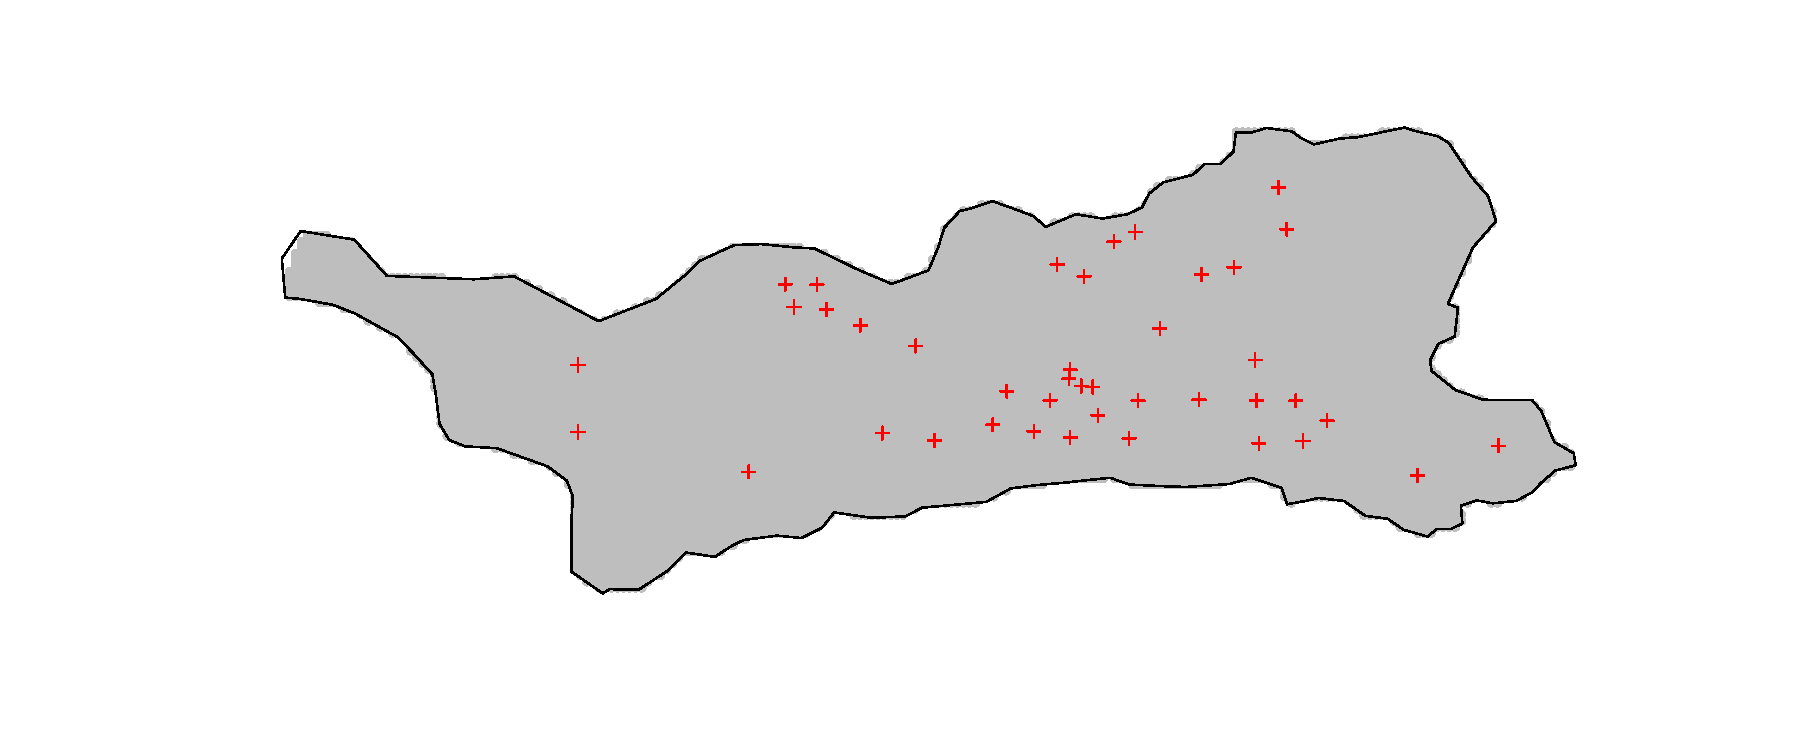
\includegraphics[width=16cm]{../ghosts/figures/Tostplot.pdf}
\caption{Tost survey mesh and traps}
\label{fig:Tostplot}
\end{centering}
\end{figure}

Fit a simple model and extract detection parameters:

\begin{Schunk}
\begin{Sinput}
> Tostfit.null <- secr.fit(Tost_ch, detectfn="HHN", mask=TostMask,model=list(D~1, lambda0~1, sigma~1),trace=0)
> detectpars = detectpar(Tostfit.null)
> l0 = detectpars$lambda0
> sig = detectpars$sigma
> tm = usage(Tost_traps) # usage
\end{Sinput}
\end{Schunk}
}

Now calculate the prob detected, prob detected only once, prob detected at least once for every mesh point, and the expected number of times an animal will be detected (just as a realioty check).

With the HHN model, the expected number of detections (assuming Poisson number of detections) of an animal at a trap with activity centre at $\mathbf{s}$ that is distance $d(\mathbf{s})$ from its activity centre is $\lambda(d(\mathbf{s})) = \lambda_0\exp(-d(\mathbf{s})^2/\sigma^2)$ and the expected number of detections of an animal at \textit{any} trap is $\lambda_\cdot = \lambda_0\exp(-\sum_j d_j(\mathbf{s})^2/\sigma^2)$, where the sum is over all traps $j=1,\ldots,J$. It follows that the probabilities that an animal with activity centre at $\mathbf{s}$ is detected at all, the probability that it is detected exactly once, and the probability that it is detected at least twice, are

\begin{eqnarray}
p_\cdot &=& 1-e^{-\lambda_\cdot} \\
p_1 &=& \lambda_\cdot e^{-\lambda_\cdot}\;\;\;\mbox{and}\\
p_{2+}&=& 1-e^{-\lambda_\cdot} - \lambda_\cdot e^{-\lambda_\cdot},
\end{eqnarray}
\noindent
respectively.


Here are a couple of functions needed to calculate prob detected only once and expected number of times an animal will be detected (only using the ``hazard half normal'' (HHN) model for simplicity for now).

\begin{Schunk}
\begin{Sinput}
> p.once.HHN = function(d,lambda0,sigma,tm) {
+   lambda = sum(tm*lambda0*exp(-d^2/sigma^2))
+   return(lambda*exp(-lambda))
+ }
> En.HHN = function(d,lambda0,sigma,tm) return(sum(tm*lambda0*exp(-d^2/sigma^2)))
\end{Sinput}
\end{Schunk}

Using those functions, lets calculate $p_\cdot$, $p_1$, and $p_{2+}$, as well as the ``coverage'' (percentage of survey region effectively surveyed, or effective survey area divided by actual survey area) in each case.

\begin{Schunk}
\begin{Sinput}
> distmat =  edist(TostMask, Tost_traps) # all distances from traps to mesh points
> coords = as.data.frame(TostMask) # make coords of mesh a data frame for use below
> p. = pdot(TostMask, Tost_traps, detectfn="HHN", detectpar=list(lambda0=l0, sigma=sig), noccasions=1) 
> p1 = apply(distmat,1,p.once.HHN,lambda0=l0,sigma=sig,tm=tm)
> Ens = apply(distmat,1,En.HHN,lambda0=l0,sigma=sig,tm=tm)
> p2plus = p. - p1
> coverage. = sum(p.)/length(p.)
> coverage2plus = sum(p2plus)/length(p.)
\end{Sinput}
\end{Schunk}

So with this detection function, we expect animals to be detected between 0 and 13.5 times, depending on where their activity centers are.

Lets have a look at plots of $p_\cdot$ and $p_{2+}$. We will do this by creating \texttt{SpatialPixelsDataFrames} and using the \texttt{sp} package to plot them:

\begin{Schunk}
\begin{Sinput}
> spts = SpatialPoints(coords=coords)
> sp. = SpatialPixelsDataFrame(spts, data=data.frame(p.=p.))
> sp2plus = SpatialPixelsDataFrame(spts, data=data.frame(p2plus=p2plus))
> pdf(h=8,w=10,file="../ghosts/figures/Tostprobplots.pdf")
> par(mfrow=c(2,1))
> plot(sp.,main=paste("p(det); coverage=",round(100*coverage.),"%",sep=""),what="image")
> plot(Tost_traps,add=TRUE)
> plot(sp2plus,main=paste("p(det at least twice); coverage=",round(100*coverage2plus),"%",sep=""),what="image")
> plot(Tost_traps,add=TRUE)
> dev.off()
\end{Sinput}
\begin{Soutput}
null device 
          1 
\end{Soutput}
\end{Schunk}


\begin{figure}
\begin{centering}
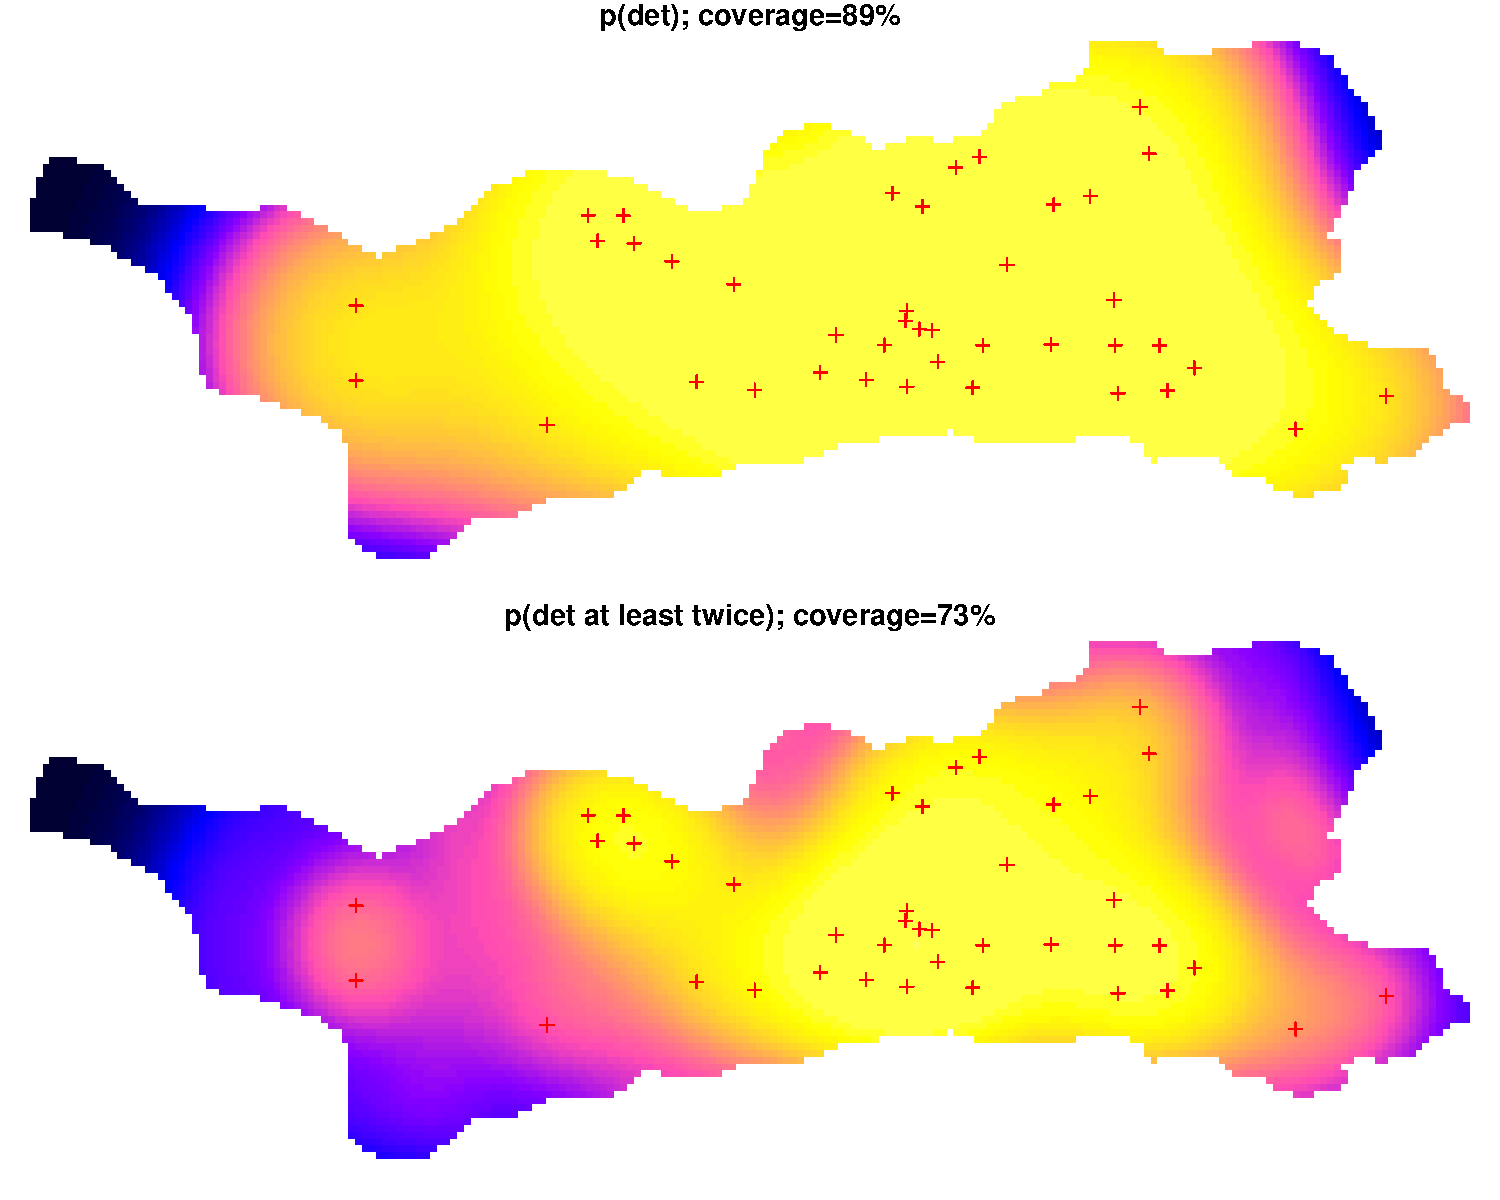
\includegraphics[width=14cm]{../ghosts/figures/Tostprobplots.pdf}
\caption{Probabilities of detection and of detection at least twice.}
\label{fig:Tostprobplots}
\end{centering}
\end{figure}

It might also be useful to look at the ratio of the coverages, which would equal to the ratio of the expected number of animals that were detected and the expected number of animals that were detected at least twice if there were no ghost detections.

\begin{Schunk}
\begin{Sinput}
> coveratio = 100*(1-coverage2plus/coverage.)
\end{Sinput}
\end{Schunk}

From which we see that you'd expect to detect about 19\% more animals than animals that were detected twice, if there were no ghosts.
\end{document}
